\documentclass[11pt,a4paper]{article}

% ==================== PACOTES ====================
\usepackage[utf8]{inputenc}
\usepackage[T1]{fontenc}
\usepackage[brazil]{babel}
\usepackage{geometry}
\geometry{top=2.0cm, bottom=2.2cm, left=2.0cm, right=2.0cm}
\usepackage{graphicx}
\usepackage{float}
\usepackage{hyperref}
\usepackage{enumitem}
\usepackage{booktabs}
\usepackage{array}
\usepackage{amssymb}
\usepackage{xcolor}
\usepackage{listings}
\usepackage{tcolorbox}
\tcbuselibrary{skins,breakable}

% ==================== CORES E ESTILOS ====================
\definecolor{imeblue}{RGB}{0, 51, 102}
\definecolor{alertred}{RGB}{180, 20, 20}
\definecolor{homegreen}{RGB}{20, 110, 50}
\definecolor{theorypurple}{RGB}{90, 40, 130}
\definecolor{armorange}{RGB}{190, 80, 10}
\definecolor{codebg}{RGB}{245, 247, 250}

\hypersetup{
    colorlinks=true,
    linkcolor=imeblue,
    urlcolor=imeblue
}

\lstset{
    backgroundcolor=\color{codebg},
    basicstyle=\ttfamily\small,
    breaklines=true,
    frame=single,
    rulecolor=\color{gray!40},
    showstringspaces=false,
    commentstyle=\color{homegreen},
    keywordstyle=\color{imeblue}\bfseries,
    literate={á}{{\'a}}1 {à}{{\`a}}1 {ã}{{\~a}}1 {â}{{\^a}}1
             {é}{{\'e}}1 {ê}{{\^e}}1 {í}{{\'i}}1 {ó}{{\'o}}1
             {õ}{{\~o}}1 {ô}{{\^o}}1 {ú}{{\'u}}1 {ç}{{\c{c}}}1
             {Á}{{\'A}}1 {É}{{\'E}}1 {Í}{{\'I}}1 {Ó}{{\'O}}1
             {Ú}{{\'U}}1 {Ç}{{\c{C}}}1
}

% Caixas didáticas personalizadas
\newtcolorbox{alertbox}[1]{
    colback=alertred!5!white,
    colframe=alertred,
    fonttitle=\bfseries,
    title={#1},
    breakable
}

\newtcolorbox{theorybox}[1]{
    colback=theorypurple!5!white,
    colframe=theorypurple,
    fonttitle=\bfseries,
    title={#1},
    breakable
}

\newtcolorbox{homebox}[1]{
    colback=homegreen!5!white,
    colframe=homegreen,
    fonttitle=\bfseries,
    title={#1},
    breakable
}

\newtcolorbox{labbox}[1]{
    colback=imeblue!5!white,
    colframe=imeblue,
    fonttitle=\bfseries,
    title={#1},
    breakable
}

\newtcolorbox{armbox}[1]{
    colback=armorange!5!white,
    colframe=armorange,
    fonttitle=\bfseries,
    title={#1},
    breakable
}

% ==================== INÍCIO DO DOCUMENTO ====================
\begin{document}

\begin{center}
    {\Large \textbf{INSTITUTO MILITAR DE ENGENHARIA (IME)}}\\[0.15cm]
    {\large Seção de Engenharia Elétrica --- SE/3}\\[0.1cm]
    {\normalsize Programação Aplicada à Engenharia Elétrica (SE/3 - Eletrônica)}\\[0.25cm]
    {\Large \textbf{Guia Mestre de Orientação e Desenvolvimento: Passos 1 e 2}}\\[0.1cm]
    {\normalsize \textit{Modelagem POO em C++, Subsistema IIO no Linux, Compilação Cruzada e Deploy Embarcado}}\\[0.35cm]
    \begin{tabular}{lp{11.0cm}}
        \toprule
        \textbf{Instituição:} & Instituto Militar de Engenharia (IME) / SE/3 \\
        \textbf{Projeto Final:} & Monitoramento Inteligente de Carga Sensível em Operações Logísticas \\
        \textbf{Kit de Desenvolvimento:} & STMicroelectronics \textbf{STM32MP157D-DK1} (Linux Embarcado OpenSTLinux) \\
        \textbf{Sensor do Grupo (Nº 3):} & Módulo de Obstáculo Infravermelho Reflexivo Digital (\textbf{HW-201} / LM393) \\
        \textbf{Passo 1 (Entrega 1):} & \textbf{26/10/2026 às 23:59} --- Classe C++ com Doxygen no Git (2,0 pts / 800 pts) \\
        \textbf{Passo 2 (Entrega 2):} & \textbf{02/11/2026 às 23:59} --- Binário ARM na Placa + README com Prints (2,0 pts / 800 pts) \\
        \bottomrule
    \end{tabular}
\end{center}

\vspace{0.2cm}

% ====================================================================
\section{Cronograma Oficial e Metas Imediatas}
% ====================================================================

Com a conclusão e aprovação da Entrega 0 (montagem física e conferência da ligação segura em 3,3 V), o projeto entra na sua fase central de desenvolvimento de software de tempo real e sistemas embarcados. A tabela abaixo sintetiza todo o ciclo avaliativo:

\begin{center}
\begin{tabular}{llcp{7.4cm}}
    \toprule
    \textbf{Etapa} & \textbf{Prazo Final} & \textbf{Pontos} & \textbf{Entregável Principal} \\
    \midrule
    \textbf{Entrega 0} & 19/10/2026 & Obrig. & Validação física da montagem com o kit desligado (Concluído). \\
    \textbf{Entrega 1} & \textbf{26/10/2026} & 2,0 pts & Classe C++ (\texttt{IrObstacleSensor}) documentada com Doxygen no GitHub. \\
    \textbf{Entrega 2} & \textbf{02/11/2026} & 2,0 pts & Executável compilado de forma cruzada rodando no Linux da placa. \\
    \textbf{Entrega 3} & 09/11/2026 & 2,0 pts & Envio contínuo das leituras via socket UDP pela interface Ethernet. \\
    \textbf{Entrega 4} & 16/11/2026 & 2,0 pts & Interface gráfica (GUI) no computador central com histórico e log CSV. \\
    \textbf{Entrega 5} & 16/11/2026 & 2,0 pts & \textbf{Mesma data da Entrega 4!} Vídeo, documentação final e integração. \\
    \bottomrule
\end{tabular}
\end{center}

\begin{alertbox}{A Regra Crítica de POO da Disciplina (Critério Eliminatório)}
O edital oficial estabelece de forma categórica: \textbf{é terminantemente proibida a utilização de variáveis globais e de funções soltas fora de classes}.
\begin{itemize}[leftmargin=*]
    \item \textbf{Por que essa regra existe?} Na Entrega 5, todos os módulos desenvolvidos pelos grupos da turma serão integrados em uma central de monitoramento. Se dois alunos criarem uma variável chamada \texttt{int valor;} ou uma função \texttt{void ler();}, ocorrerá colisão de símbolos no momento da ligação (\textit{linker error}).
    \item \textbf{A solução correta:} Todo estado (caminho de arquivos, limiares, histórico) deve ser atributo \texttt{private} da classe, acessível apenas por métodos \texttt{public} devidamente documentados.
\end{itemize}
\end{alertbox}

\newpage
% ====================================================================
\section{MÓDULO 1 (Passo 1): Modelagem C++, Linux IIO e Doxygen}
% ====================================================================

\subsection{A Teoria: Como o Linux Embarcado Trata os Pinos Físicos?}
A placa STM32MP157D-DK1 não roda o código em modo microcontrolador puro (\textit{bare-metal}). Ela executa uma distribuição Linux completa baseada em Buildroot/OpenSTLinux. No ambiente Linux, vigora o paradigma universal: \textbf{``Tudo é um arquivo'' (\textit{Everything is a file})}.

\begin{theorybox}{O Subsistema IIO (Industrial I/O)}
Para permitir que programas em espaço de usuário (\textit{user space}) acessem conversores Analógico-Digitais (ADC), acelerômetros e sensores industriais de forma padronizada e segura, o Kernel do Linux expõe o subsistema \textbf{IIO} através do sistema de arquivos virtual \texttt{sysfs}:
\begin{center}
    \texttt{/sys/bus/iio/devices/iio:device0/}
\end{center}
Dentro desse diretório virtual, o driver de hardware cria arquivos como \texttt{in\_voltage0\_raw}, \texttt{in\_voltage1\_raw}, etc.
Quando o seu programa em C++ abre esse arquivo e lê o seu conteúdo, o Kernel realiza a conversão A/D instantânea no pino físico da placa e devolve o valor como um número inteiro em formato texto (por exemplo, \texttt{0} para 0 V ou \texttt{4095}/\texttt{65535} para 3,3 V).
\end{theorybox}

\subsection{Passo Presencial (Laboratório): Descobrir o Canal Exato do ADC}
Na Entrega 0, o fio de sinal do seu sensor foi conectado no \textbf{Pino 5 do conector de 6 furos (ADC)}. Agora, no laboratório, você precisa descobrir qual número \texttt{X} corresponde a esse pino físico.

\begin{figure}[H]
    \centering
    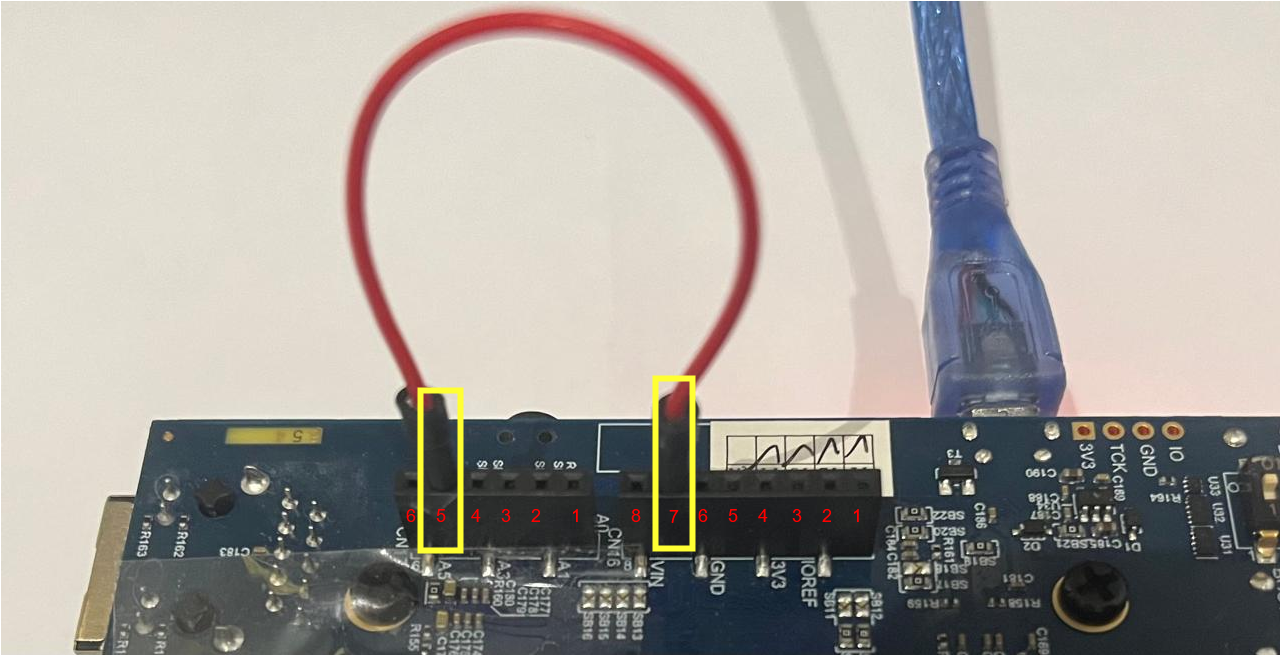
\includegraphics[width=0.62\textwidth]{latex_assets/page8_img1.png}
    \caption{Procedimento oficial de descoberta de canal: Jumper ligando diretamente o Pino 5 do ADC ao GND (Pino 6/7) para forçar leitura zero no canal correspondente.}
\end{figure}

\begin{labbox}{Procedimento de 5 Minutos no Laboratório}
\begin{enumerate}[leftmargin=*]
    \item \textbf{Aterrar o pino de leitura:} Com a placa desligada, retire temporariamente o fio do sensor do Pino 5 do bloco ADC e coloque um jumper conectando o \textbf{Pino 5} diretamente ao \textbf{Pino 7 (GND)} do bloco de alimentação.
    \item \textbf{Energizar e conectar a Serial:}
    \begin{itemize}
        \item Conecte o cabo USB-C na porta \texttt{PWR\_IN}.
        \item Conecte o cabo Micro-USB na porta serial \texttt{ST-LINK} e abra o TeraTerm/PuTTY configurado para \textbf{115200 8N1}.
        \item Pressione Enter e efetue login com usuário \texttt{root} e senha \texttt{root}.
    \end{itemize}
    \item \textbf{Consultar os canais IIO no terminal:}
\begin{lstlisting}[language=bash]
cd /sys/bus/iio/devices/iio:device0/
cat in_voltage*_raw
\end{lstlisting}
    \item \textbf{Identificação:} O arquivo \texttt{in\_voltageX\_raw} que retornar o valor \textbf{0} (ou ruído elétrico quase nulo, ex.: 1 ou 2) é o canal exato do seu sensor!
    \item \textbf{Teste com o Sensor HW-201:} Desligue a placa, retire o jumper de aterramento e reconecte os 3 fios do sensor HW-201. Ao ligar e ler o arquivo identificado:
    \begin{itemize}
        \item Com o compartimento livre (sem reflexão): leitura alta (nível lógico ALTO $\approx$ 3,3 V).
        \item Com a tampa fechada/mão próxima: o feixe reflete, a saída vai para nível BAIXO e a leitura cai para valores próximos de zero.
    \end{itemize}
\end{enumerate}
\end{labbox}

\subsection{Passo em Casa: Simulando o Hardware no seu Computador}
Você não precisa da placa física para desenvolver, depurar e testar 100\% da sua classe C++. Como a leitura ocorre através de um arquivo de texto, você pode criar um simulador local no seu computador (Linux, WSL ou terminal Git Bash):

\begin{homebox}{Criando o Ambiente de Teste Caseiro}
\begin{lstlisting}[language=bash]
# 1. Cria diretorio simulando a estrutura sysfs do Linux
mkdir -p /tmp/mock_iio

# 2. Simula o estado NORMAL (tampa fechada / feixe refletindo -> 0V)
echo "150" > /tmp/mock_iio/in_voltage0_raw

# 3. Simula o estado de VIOLACAO (tampa aberta / sem reflexao -> 3.3V)
echo "4050" > /tmp/mock_iio/in_voltage0_raw
\end{lstlisting}
Projetando a sua classe para aceitar o caminho do arquivo no construtor (com valor padrão apontando para a placa real), o mesmo código compilará e executará tanto no seu PC em casa quanto na placa no laboratório!
\end{homebox}

\subsection{Modelando a Classe C++ (\texttt{IrObstacleSensor})}
A estrutura deve seguir estritamente o padrão da engenharia de software moderna em C++: divisão entre o contrato de interface (\texttt{include/IrObstacleSensor.hpp}) e a implementação dos métodos (\texttt{src/IrObstacleSensor.cpp}).

\begin{theorybox}{Estrutura do Cabeçalho (\texttt{include/IrObstacleSensor.hpp})}
\begin{lstlisting}[language=C++]
#ifndef IR_OBSTACLE_SENSOR_HPP
#define IR_OBSTACLE_SENSOR_HPP

#include <string>

/**
 * @file IrObstacleSensor.hpp
 * @brief Classe de aquisicao e interpretacao do Sensor de Obstaculo IR HW-201.
 */
class IrObstacleSensor {
private:
    std::string devicePath;  /**< Caminho do arquivo IIO no sysfs ou arquivo mock */
    int rawThreshold;        /**< Limiar de comutacao entre estado normal e violacao */
    int lastRawValue;        /**< Ultima leitura numerica bruta obtida do conversor ADC */
    double referenceVoltage; /**< Tensao de referencia do circuito (3.3 V) */
    int maxAdcResolution;    /**< Resolucao maxima da escala do conversor (ex: 4095) */

public:
    /**
     * @brief Construtor da classe com parametros padrao configuraveis.
     * @param path Caminho do arquivo sysfs IIO ou arquivo mock para testes em casa.
     * @param threshold Limiar de decisao logica entre nivel alto e baixo.
     * @param vref Tensao de alimentacao de referencia em Volts (3.3V).
     * @param maxAdc Escala maxima do conversor A/D (4095 para 12 bits).
     */
    explicit IrObstacleSensor(
        const std::string& path = "/sys/bus/iio/devices/iio:device0/in_voltage0_raw",
        int threshold = 2000,
        double vref = 3.3,
        int maxAdc = 4095
    );

    int readRaw();                     /**< Realiza a leitura atomica do arquivo IIO */
    double getVoltage() const;         /**< Converte a leitura bruta em tensao (Volts) */
    bool isObstacleDetected() const;   /**< Retorna true se houver reflexao (Active-Low) */
    bool isCompartmentViolated() const;/**< Avalia a integridade da carga monitorada */
    int getLastRawValue() const;       /**< Retorna o ultimo valor lido */
    void setThreshold(int newThreshold);/**< Ajuste dinamico do limiar de alerta */
};

#endif // IR_OBSTACLE_SENSOR_HPP
\end{lstlisting}
\end{theorybox}

\begin{theorybox}{Implementação dos Métodos (\texttt{src/IrObstacleSensor.cpp}) e Princípio RAII}
Ao manipular arquivos no Linux com C++, a biblioteca padrão \texttt{<fstream>} aplica o conceito de \textbf{RAII (\textit{Resource Acquisition Is Initialization})}:
\begin{lstlisting}[language=C++]
#include "IrObstacleSensor.hpp"
#include <fstream>
#include <stdexcept>

IrObstacleSensor::IrObstacleSensor(const std::string& path, int threshold, double vref, int maxAdc)
    : devicePath(path), rawThreshold(threshold), lastRawValue(0),
      referenceVoltage(vref), maxAdcResolution(maxAdc) {}

int IrObstacleSensor::readRaw() {
    std::ifstream file(devicePath);
    if (!file.is_open()) {
        throw std::runtime_error("Falha ao abrir canal IIO no caminho: " + devicePath);
    }
    file >> lastRawValue;
    return lastRawValue; // O arquivo eh fechado automaticamente pelo destrutor de ifstream!
}

bool IrObstacleSensor::isObstacleDetected() const {
    // Sensor HW-201 com comparador LM393 opera em Active-Low:
    // Reflexao detectada (objeto proximo) -> Saida comuta para nivel BAIXO (0V / ADC proximo a 0)
    return lastRawValue < rawThreshold;
}

bool IrObstacleSensor::isCompartmentViolated() const {
    // No contexto da carga: se o feixe nao reflete na tampa, o compartimento foi violado!
    return !isObstacleDetected();
}
\end{lstlisting}
\end{theorybox}

\subsection{Documentação com Doxygen e Submissão da Entrega 1}
O edital exige documentação completa da classe via Doxygen:
\begin{enumerate}[leftmargin=*]
    \item \textbf{Tags fundamentais:} \texttt{@file} (descrição do arquivo), \texttt{@class} (escopo da classe), \texttt{@brief} (resumo sucinto do método), \texttt{@param} (significado dos parâmetros recebidos) e \texttt{@return} (valor de retorno).
    \item \textbf{Geração do Doxyfile:} Execute \texttt{doxygen -g Doxyfile} no terminal. Edite as linhas:
    \begin{itemize}
        \item \texttt{INPUT = include src}
        \item \texttt{EXTRACT\_PRIVATE = YES} (para documentar também os atributos privados).
    \end{itemize}
    \item \textbf{Geração e Validação:} Execute \texttt{doxygen Doxyfile} e abra \texttt{html/index.html} no navegador.
    \item \textbf{Envio do Link do Commit:} Faça o commit no Git, envie com \texttt{git push origin main}, abra o GitHub no navegador, clique na aba \textbf{Commits}, selecione o commit gerado e envie a URL direta no Google Classroom!
\end{enumerate}

\newpage
% ====================================================================
\section{MÓDULO 2 (Passo 2): Compilação Cruzada e Deploy Embarcado}
% ====================================================================

A \textbf{Entrega 2 (02/11/2026)} consiste em gerar o executável final funcional, rodando diretamente no Linux embarcado da placa STM32MP157D-DK1, lendo o sensor físico e com instruções e prints devidamente documentados no \texttt{README.md}.

\subsection{Fundamentos de Compilação Cruzada (\textit{Cross-Compilation})}
\begin{armbox}{Por que não podemos compilar com o \texttt{g++} comum do PC?}
O processador do seu computador é da arquitetura \textbf{x86\_64 (Intel/AMD)}, com um conjunto de instruções específico. Já o processador da sua placa STM32MP157D-DK1 é um \textbf{Dual-core Arm Cortex-A7 (ARMv7-A de 32 bits)} com ponto flutuante via hardware (\texttt{vfpv4-d16 / neon}).
\begin{itemize}[leftmargin=*]
    \item Se você compilar no PC com o \texttt{g++} nativo, o binário conterá instruções x86\_64 que o processador ARM da placa não é capaz de decodificar (resultando em erro imediato de execução: \textit{``cannot execute binary file: Exec format error''}).
    \item Para resolver isso, utilizamos uma \textbf{Toolchain de Compilação Cruzada}, na qual o compilador roda no seu computador x86\_64 (\textit{Host}), mas traduz a sintaxe C++ gerando código de máquina ARM (\textit{Target}).
\end{itemize}
\end{armbox}

\subsection{Configuração da Toolchain no Linux}
O projeto disponibiliza duas opções de ambiente de compilação cruzada no repositório:
\begin{enumerate}[leftmargin=*]
    \item \textbf{Opção A: Toolchain Buildroot (\texttt{arm-buildroot-linux-gnueabihf\_sdk-DK2.tar.gz}):}
    \begin{lstlisting}[language=bash]
# Extrair o pacote da toolchain no seu diretorio de desenvolvimento
tar -xvf arm-buildroot-linux-gnueabihf_sdk-DK2.tar.gz

# Localizar o compilador g++ dentro da pasta extraida:
export PATH=$PATH:/caminho/da/toolchain/bin
arm-buildroot-linux-gnueabihf-g++ --version
    \end{lstlisting}
    \item \textbf{Opção B: SDK Yocto OpenSTLinux (\texttt{SDK-x86\_64-stm32mp1-...}):} \\
    Permite inicializar as variáveis de ambiente completas com suporte ao \textit{sysroot} da placa.
\end{enumerate}

\subsection{Automação Profissional com \texttt{Makefile}}
Para garantir reprodutibilidade e atender às exigências de compilação documentadas no edital, crie um \texttt{Makefile} na raiz do projeto com alvos bem definidos:

\begin{theorybox}{Estrutura do \texttt{Makefile} para Compilação Híbrida (PC e ARM)}
\begin{lstlisting}[language=make]
# Compilador nativo (para testes locais no PC em casa)
CXX ?= g++
CXXFLAGS = -Wall -Wextra -std=c++17 -Iinclude -O2

# Toolchain de Cross-Compilacao (para o processador ARM da STM32MP1)
CROSS_PREFIX ?= arm-buildroot-linux-gnueabihf-
CROSS_CXX = $(CROSS_PREFIX)g++

SRCS = src/IrObstacleSensor.cpp src/main.cpp
TARGET_NATIVE = app_sensor
TARGET_ARM = app_sensor_arm

.PHONY: all cross clean doc

all: $(TARGET_NATIVE)

$(TARGET_NATIVE): $(SRCS)
	$(CXX) $(CXXFLAGS) -o $@ $^
	@echo "Binario nativo para PC gerado com sucesso!"

cross: $(SRCS)
	$(CROSS_CXX) $(CXXFLAGS) -o $(TARGET_ARM) $^
	@echo "Binario cross-compilado para ARM Cortex-A7 gerado com sucesso!"

doc:
	doxygen Doxyfile

clean:
	rm -f $(TARGET_NATIVE) $(TARGET_ARM) *.o
\end{lstlisting}
\end{theorybox}

\subsection{Teste Caseiro do Binário ARM com QEMU (\textit{User Mode})}
Você pode verificar se a compilação cruzada foi bem-sucedida sem precisar esperar pelo laboratório. O emulador QEMU permite rodar binários de outras arquiteturas no seu próprio PC Linux:
\begin{lstlisting}[language=bash]
# 1. Instalar o suporte ao QEMU User Space na sua maquina Linux
sudo apt update && sudo apt install -y qemu-user qemu-user-static

# 2. Executar o binario ARM apontando para o sysroot da toolchain
qemu-arm -L /caminho/da/toolchain/arm-buildroot-linux-gnueabihf/sysroot ./app_sensor_arm /tmp/mock_iio/in_voltage0_raw
\end{lstlisting}
Se o binário rodar sem falhas no QEMU, a execução física na placa STM32MP157D-DK1 funcionará de primeira.

\subsection{Procedimento de Bancada: Rede, Transferência e Execução Remota}
No laboratório, a comunicação entre o computador e a placa é realizada através de um cabo de rede Ethernet comum (RJ45):

\begin{figure}[H]
    \centering
    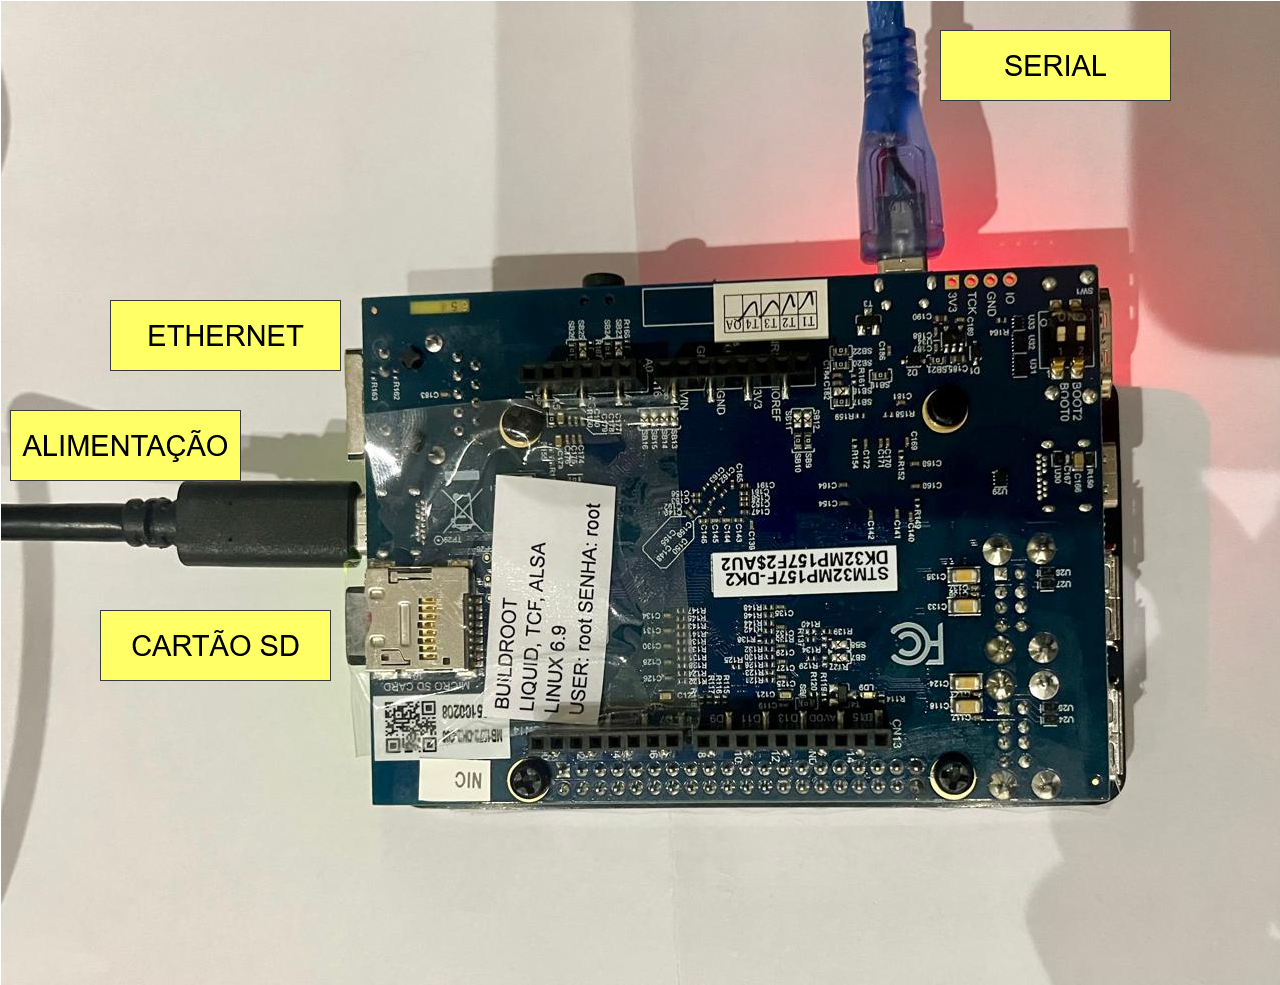
\includegraphics[width=0.70\textwidth]{latex_assets/page6_img1.png}
    \caption{Porta Ethernet da placa STM32MP157D-DK1 (ao lado da entrada USB-C de alimentação).}
\end{figure}

\begin{labbox}{Roteiro de Bancada para a Entrega 2}
\begin{enumerate}[leftmargin=*]
    \item \textbf{Conexão Física e Alimentação:}
    \begin{itemize}
        \item Conecte o cabo USB-C na porta \texttt{PWR\_IN}.
        \item Conecte o cabo de rede Ethernet entre a placa e a porta de rede do computador.
        \item Certifique-se de que os 3 fios do sensor HW-201 permanecem conectados nos pinos validados na Entrega 0 (Pino 4 = 3V3, Pino 7 = GND, Pino 5 = ADC).
    \end{itemize}
    \item \textbf{Configuração da Rede Local no PC:}
    \begin{itemize}
        \item A placa STM32MP157D-DK1 possui o endereço IP fixo configurado no laboratório: \textbf{\texttt{192.168.42.2}}.
        \item No seu computador, abra as configurações de rede da interface Ethernet e defina um IP estático na mesma sub-rede, por exemplo:
        \begin{itemize}
            \item IP do Computador: \textbf{\texttt{192.168.42.10}}
            \item Máscara de Sub-rede: \textbf{\texttt{255.255.255.0}}
            \item Gateway: \textit{Pode deixar em branco}.
        \end{itemize}
    \end{itemize}
    \item \textbf{Transferir o Binário via SCP (\textit{Secure Copy}):} \\
    No terminal do seu computador (onde você gerou o arquivo \texttt{app\_sensor\_arm}), envie o programa para a pasta \texttt{/home/root} da placa:
\begin{lstlisting}[language=bash]
scp app_sensor_arm root@192.168.42.2:/home/root/
\end{lstlisting}
    \textit{Quando solicitar a senha, digite \texttt{root}.}
    
    \item \textbf{Acessar a Placa via SSH e Executar o Programa:}
\begin{lstlisting}[language=bash]
# Acessa o shell Linux da placa remotamente via rede
ssh root@192.168.42.2

# Entra na pasta e concede permissao de execucao
cd /home/root
chmod +x app_sensor_arm

# Executa o programa lendo o sensor fisico real
./app_sensor_arm
\end{lstlisting}
\end{enumerate}
\end{labbox}

\subsection{Calibração Prática do Sensor HW-201}
Com o programa rodando e exibindo as leituras em tempo real no terminal da placa:
\begin{itemize}[leftmargin=*]
    \item \textbf{Ajuste do Trimpot:} Utilize uma chave de fenda pequena no potenciômetro quadrado azul do sensor HW-201. Gire até que o LED verde do sensor acenda exatamente quando a tampa do baú/obstáculo estiver na distância planejada (entre 5 cm e 15 cm).
    \item \textbf{Registro de Evidências (Prints):}
    \begin{itemize}
        \item Tire um print do terminal mostrando as leituras contínuas com a \textbf{tampa fechada / compartimento seguro} (valores baixos de ADC).
        \item Abra o compartimento e tire um print imediato mostrando a comutação para \textbf{alarme de violação} (valores altos de ADC).
    \end{itemize}
\end{itemize}

\subsection{Requisitos do \texttt{README.md} para a Entrega 2}
Conforme a Instrução Geral nº 5 do edital, o arquivo \texttt{README.md} deve ser atualizado com:
\begin{enumerate}[leftmargin=*]
    \item Instruções exatas e reproduzíveis do comando de compilação cruzada.
    \item Comando de transferência via \texttt{scp} e de execução via \texttt{ssh}.
    \item Imagens/prints do terminal anexados na pasta \texttt{docs/} mostrando a aplicação em funcionamento real.
    \item Submissão do link do commit final da Entrega 2 no Google Classroom até \textbf{02/11/2026 às 23:59}.
\end{enumerate}

\newpage
% ====================================================================
\section{MÓDULO 3: Visão Geral das Etapas Subsequentes}
% ====================================================================

Para que o desenvolvimento do grupo mantenha coerência arquitetural desde os Passos 1 e 2, este é o horizonte das fases seguintes:

\begin{center}
\begin{tabular}{lp{12.0cm}}
    \toprule
    \textbf{Etapa} & \textbf{Conceitos-Chave e Desafios de Engenharia} \\
    \midrule
    \textbf{Passo 3 (09/11):} & \textbf{Telemetria via Socket UDP em C++ (POSIX):} \\
    & Criação de uma classe modular (ex.: \texttt{UdpTransmitter}) utilizando as bibliotecas de sistema \texttt{<sys/socket.h>} e \texttt{<arpa/inet.h>}. O programa embarcado na STM32MP1 enviará datagramas contínuos contendo identificador do sensor, estado da carga e timestamp para a porta UDP do computador central. \\
    \midrule
    \textbf{Passo 4 (16/11):} & \textbf{Interface Gráfica de Monitoramento no Computador (GUI):} \\
    & Desenvolvimento de dashboard no PC em Python (PyQt / Matplotlib / PyQtGraph) ou C++/Qt. A interface escuta na porta UDP, plota gráfico deslizante de 30 a 60 segundos com taxa de atualização fluida, exibe alerta visual de invasão e exporta logs em arquivo CSV. \\
    \midrule
    \textbf{Passo 5 (16/11):} & \textbf{Documentação Consolidada, Vídeo e Simulação Integrada:} \\
    & Produção do vídeo demonstrativo mostrando o hardware operando de ponta a ponta (atuação física no sensor $\rightarrow$ reação imediata na tela do PC), refinamento do diagrama UML no \texttt{README.md} e participação no teste conjunto com os 11 sensores da turma. \\
    \bottomrule
\end{tabular}
\end{center}

\vspace{0.4cm}
\begin{center}
    \rule{0.6\textwidth}{0.4pt}\\[0.2cm]
    {\small \textbf{SE/3 --- Eletrônica --- Programação Aplicada à Engenharia Elétrica --- IME 2026}}
\end{center}

\end{document}
